
\section{Prototype}
\label{sec:prototype}

\begin{figure}[t]
	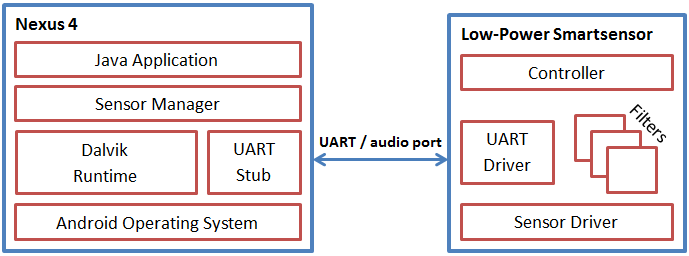
\includegraphics[width=8.5cm]{prototype_architecture.png}
	\caption{High-level architecture of our prototype implementation}
    \label{fig:prototypeArchitecture}
\end{figure}

We implemented a prototype of our system using a Google Nexus 4 running Android 4.2.2. The low-power smart sensor is implemented using a Texas Instruments micro-controller board attached to an accelerometer sensor. The Nexus 4 and TI board communicate over the UART port made available by the Nexus 4 debugging interface. Figure \ref{fig:prototypeArchitecture} shows a high-level diagram of the prototypes architecture.

We chose to focus our efforts on the accelerometer sensor because of its relative simplicity and the availability of a wide range of accelerometer-based applications on various mobile application markets. Nevertheless, the approach can be extended to other sensors such as the microphone, GPS or WiFi. However, extending the prototype to work with higher bandwidth sensors like the camera would require a higher bandwidth data bus such as $I^2C$. 


\subsection{Google Nexus 4}

\begin{figure*}[t]
	\begin{verbatim}
		SensorManager mSensorManager = (SensorManager) getSystemService(Context.SENSOR_SERVICE);
		Sensor mAccelerometer = mSensorManager.getDefaultSensor(Sensor.TYPE_ACCELEROMETER);
		mSensorManager.registerListener(new MySensorEventListener(), mAccelerometer);
	\end{verbatim}
	\caption{Typical usage of Android's SensorManager}
    \label{fig:androidSensorCodeNormal}
\end{figure*}

\begin{figure*}[t]
	\begin{verbatim}
		SensorManager mSensorManager = (SensorManager) getSystemService(Context.SENSOR_SERVICE);
		Sensor mAccelerometer = mSensorManager.getDefaultSensor(Sensor.TYPE_ACCELEROMETER);
		WakeUpCondition mWakeUpCondition = new MinThresholdWakeUpCondition(Sensor.AXIS_X, 12.0);
		mSensorManager.registerListener(new MySensorEventListener(), mAccelerometer, mWakeUpCondition);
	\end{verbatim}
	\caption{Usage of the SensorManager with a wakeup condition}
    \label{fig:androidSensorCodeModified}
\end{figure*}

On the Nexus phone we extended Android's SensorManager to include the new features made available by our system. To prevent a steep learning curve, our goal was to provide an API very similar to Android's existing sensors API. Normally, in order to receive sensor data, an application needs to register a listener (i.e. an implementation of the SensorEventListener interface) for a specific sensor with Android's SensorManager. Figure \ref{fig:androidSensorCodeNormal} shows a code example of a typical application registering a listener with the Android SensorManager for accelerometer readings. We extended the Sensor Manager to include functions that take an additional parameter that specifies which wake-up condition to be used. The available types of wakeup conditions, described in detail in Subsection \ref{sec:sensorDataFilters}, are a set predefined implementations of a WakeUpCondition interface. Figure \ref{fig:androidSensorCodeModified} shows an example of the modified code to include a wakeup condition that is satisfied when the raw x-axis acceleration exceeds $12 m/s^2$.

We also created a UART stub to facilitate the communication between the mobile phone and the smart sensor board. The UART stub is called when the smart sensor board detects an event based on its wakeup condition. In turn, the UART stub notifies the SensorManager using an Android Intent(TODO: reference to Android Intent documentation?).

For our prototype we did not have to modify the operating system on the phone in any way. Because the current prototype uses the UART port for communication with the smart sensor, we were able to constrain our implementation to the user space. An integrated implementation would very likely make use of the higher bandwidth bus such as the $I^2C$ and require a custom driver and possibly modification to the operating system.

\begin{table*}[t]
	\begin{tabular}{| p{7cm} | l | l |}
		\hline
		State & Average Power Consumption (mW) & Average Duration \\ \hline
	%    TI MSP430 & Awake & 3.6 & N/A \\ \hline
	%    TI Stellaris & Awake & 49.4 & N/A \\ \hline
		Awake, running a pedometer application with data from the internal accelerometer & 323 & N/A \\ \hline
		Asleep & 9.7 & N/A \\ \hline
		Asleep-to-Awake Transition & 384 & 1 second \\ \hline
		Awake-to-Asleep Transition & 341 & 1 second \\ \hline
	\end{tabular}
	\caption{Power Profile for the Google Nexus 4}
	\label{table:powerProfileNexus}
\end{table*}

We power profiled the Google Nexus 4. The results are summarized in Table \ref{table:powerProfileNexus}. During all the measurements, the device's screen was turned off. Additionally, we noticed that changes in signal strength for GSM, WiFi and GPS resulted in fluctuations in the power consumption of the device. To prevent these factors from affecting our power profile, we decided to run all the power measurements with GSM, WiFi and GPS turned off. While the device is sleeping, its power consumption is very low, consuming only 9.7 mW. While awake, the power consumption is significantly higher, averaging 323 mW. During our power measurements we noticed that additional energy is consumed during transitions between the asleep and awake states. Each transition takes about 1 second. During a wakeup transition, the average power consumption goes up to 384 mW, while during an awake-to-asleep transition the average power consumption rises to 341 mW.


\subsection{Smart Sensor Board}

On the low-power smart sensor board, the prototype consists of a driver that talks to the accelerometer sensor, a set of filtering algorithms, a controller, and an UART driver for communicating with the phone. The controller orchestrates the execution of the filters, and uses the UART driver to wake up the phone when a wakeup condition is satisfied. The UART driver is in charge of waking up the phone, running a shell program that issues a Android Intent to start the UART stub, and passing the sensor readings to the main device. 

\subsubsection{Sensor Data Filters}
\label{sec:sensorDataFilters}

We implemented three types of sensor data filters (or wakeup conditions) of varying complexities. All wakeup conditions are based on thresholding over some accelerometer readings. The wakeup conditions differ in what readings are checked against the threshold value.

The \emph{raw acceleration wakeup condition} is the simplest and requires the least amount of computation. The wakeup condition is satisfied if the raw acceleration exceeds the threshold. The threshold value is the only parameter for this wakeup condition. In our preliminary tests, we noticed that accelerometer data is particularly noisy. Our expectation was that a simple threshold filter over raw acceleration readings would be satisfied more frequently than necessary because of the noise present in the sensor data, potentially causing unnecessary device wake ups. 

The \emph{EMA LPF wakeup condition} removes some of the noise from the sensor data and is computationally cheap, requiring only several algebraic operations for every sensor reading. In this wakeup condition the raw accelerometer data is passed through a low-pass filter based on an exponential moving average before being checked against the threshold. The two parameters that can be set for this wakeup condition are the threshold value and an alpha value between 0 and 1. The alpha value controls the "smoothness" of the filtered data (TODO: rephrase).

The \emph{FFT LPF wakeup condition} is more accurate at removing noise from the sensor data. However, it is computationally expensive. In this wakeup condition the raw accelerometer data is passed through a low-pass filter based on Fast Fourier Transformations before being checked against the threshold. Two parameters can be set for this wakeup condition: the threshold value and a relative energy level value. The relative energy value indicates the percentage of the original energy present in the raw acceleration that is to be removed during filtering.  

\subsubsection{Hardware Options}

We evaluated two options as our low-powered sensor platform. 

Our first option is a Texas Instruments MSP430 micro-controller. It has the advantage of being very low-power, consuming only 3.6 mW while awake. However, it has limited memory and cannot perform complex analysis of sensor data in real-time. In our tests, the MSP430 was unable to run the Fast Fourier Transformations necessary for low-pass filtering sensor data in real-time. 

Our second option is a Texas Instruments Stellaris LM4F120H5QR micro-controller powered by a Cortex-M4 processor. It can batch a higher number of accelerometer readings and run all our wakeup conditions in real-time, including the one using FFT-based low-pass filtering. However, this micro-controller has an energy footprint an order of magnitude greater than the MSP430, consuming an average of 49.4 mW while awake.


